\documentclass[14pt, a4paper]{extreport}
\usepackage{extsizes}
\usepackage[a4paper, left=30mm, right=15mm, top=20mm, bottom=20mm]{geometry}
\usepackage[english, russian]{babel}
\usepackage{fontspec}
\defaultfontfeatures{Ligatures={TeX},Renderer=Basic}
\setmainfont[Ligatures={TeX,Historic}]{Times New Roman}
\usepackage{amsmath,amssymb}
\usepackage{graphicx}
\usepackage{setspace}
\graphicspath{{images/}}
\usepackage[hidelinks]{hyperref}
\usepackage{indentfirst}
\setlength{\parindent}{1.25cm}
\usepackage[explicit,compact]{titlesec}
\usepackage{titletoc}
\newcommand{\doublerule}[1][.4pt]{%
	\noindent
	\makebox[0pt][l]{\rule[.6ex]{\linewidth}{#1}}%
	\rule[.3ex]{\linewidth}{#1}
}

\addto\captionsrussian{%
	\renewcommand{\contentsname}%
	{\centering{СОДЕРЖАНИЕ}}%
}

\usepackage{caption}
\DeclareCaptionLabelSeparator{dash}{ -- }
\DeclareCaptionLabelFormat{figure}{Рисунок #2}
\captionsetup[table]{
	labelsep=dash,
	singlelinecheck=false,
}
\captionsetup[figure]{
	labelsep=dash,
	labelformat=figure,
}

\usepackage{floatrow}
\floatsetup[table]{style=plaintop}
\floatsetup[equation]{style=plain}

\usepackage{chngcntr}
\counterwithout{figure}{chapter}
\counterwithout{equation}{chapter}
\counterwithout{table}{chapter}

\usepackage{cleveref}
\crefformat{table}{смотри табл.#2#1#3}
\Crefformat{table}{Смотри табл.#2#1#3}

\crefformat{figure}{рис.~#2#1#3}
\Crefformat{figure}{Рис.~#2#1#3}
\crefmultiformat{figure}{рис.~#2#1#3}{,~#2#1#3}{,~#2#1#3}{,~#2#1#3}
\crefrangeformat{figure}{рис.~#3#1#4--#5#2#6}

\crefformat{equation}{#1}
\crefmultiformat{equation}{~#2#1#3}{,~#2#1#3}{,~#2#1#3}{,~#2#1#3}
\crefrangeformat{equation}{~#3#1#4--#5#2#6}

\begin{document}
\begin{titlepage}
	\begin{center}
		\vspace*{0.5mm}
		\setstretch{1.1}

		
\includegraphics[width=0.18\textwidth]{logo}\\
		\footnotesize
		МИНИСТЕРСТВО НАУКИ И ВЫСШЕГО ОБРАЗОВАНИЯ РОССИЙСКОЙ ФЕДЕРАЦИИ\\
		\small
		Федеральное государственное бюджетное образовательное учреждение высшего образования\\
		\textbf{«МИРЭА - Российский технологический университет»}
		\vspace{0.5cm}

		\large \textbf{РТУ МИРЭА} \normalsize

		\doublerule[1pt]\\
		\vspace{0.4cm}

		Институт искусственного интеллекта\\
		Кафедра общей информатики
		\vspace{1.5cm}

		\textbf{ОТЧЕТ}\\
		\textbf{ПО ПРАКТИЧЕСКОЙ РАБОТЕ № 7}\\
		\textbf{реализация заданной логической функции от четырех переменных на дешифраторах 4-16, 3-8 и 2-4}\\
		\textbf{по дисциплине}\\
		«ИНФОРМАТИКА»
		\vspace{1.5cm}

		\small
		Выполнил студент группы ИМБО-01-22 \hfill Скирдин Никита Сергеевич
		\vspace{1cm}

		Принял \hfill Павлова Екатерина Сергеевна\\
		ассистент \hfill
		\vspace{1.5cm}

		\footnotesize
		\hspace{0.5cm} Практическая \hfill «\_\_»\_\_\_\_\_\_2022 г. \hfill Подпись студента\\
		\hspace{0.5cm} работа выполнена \hfill
		\vspace{0.5cm}

		\hspace{2cm} «Зачтено» \hfill «\_\_»\_\_\_\_\_\_2022 г. \hfill Подпись преподавателя
		\vfill

		\small
		Москва 2022
	\end{center}
	\thispagestyle{empty}
\end{titlepage}

\setstretch{1.5}
\setcounter{page}{2}

\titlecontents{chapter}[0em]
	{\vskip 0.5ex}%
	{\thecontentslabel \space \uppercase}% numbered sections formatting
	{}% unnumbered sections formatting
	{\hfill \thecontentspage}%

\titlecontents{section}[1.25cm]
	{\vskip 0.5ex}%
	{\thecontentslabel \space}
	{}
	{\hfill \thecontentspage}

\titleformat{\chapter}[block]
	{\bfseries\normalsize}{}{0pt}{\uppercase{#1}}

\titleformat{\section}[block]
	{\bfseries\normalsize}{}{0pt}{#1}

\titlespacing*{\chapter}{0pt}{-10.5mm}{0pt}

\tableofcontents

\titleformat{\chapter}[display]
	{\centering\bfseries\normalsize}{}{0pt}{\thechapter \space \uppercase{#1}}

\titleformat{\section}[block]
	{\hspace{\parindent}\bfseries\normalsize}{}{0pt}{\thesection \space #1}

\titlespacing*{\chapter}{0pt}{-19.5mm}{0pt}

\chapter{Постановка задачи}
Логическая функция от четырех переменных задана в 16-теричной векторной форме. Восстановить таблицу истинности. По таблице истинности реализовать в лабораторном комплексе логическую функцию на дешифраторах тремя способами:

– используя дешифратор 4-16 и одну дополнительную схему «или»;

– используя два дешифратора 3-8 и необходимую дополнительную логику;

– используя пять дешифраторов 2-4 и одну дополнительную схему «или».

Протестировать работу схем и убедиться в правильности их работы. Подготовить отчет о проделанной работе и защитить ее.

\section{Персональный вариант}
Логическая функция от четырех переменных, заданная в 16-теричной форме: F9AA$_{16}$

\chapter{Проектирование и реализация}
\section{Предварительная подготовка данных}
Преобразуем заданную логическую функцию в двоичную запись: 1111 1001 1010 1010$_2$ - получили столбец значений логической функции, который необходим для восстановления полной таблицы истинности (\cref{tab:function-values}).

\begin{table}[!htbp]
	\caption{Таблица истинности заданной функции}
	\label{tab:function-values}
	\begin{tabular}{|c|c|c|c|c|}
		\hline
		a & b & c & d & F \\
		\hline
		0 & 0 & 0 & 0 & 1 \\
		\hline
		0 & 0 & 0 & 1 & 1 \\
		\hline
		0 & 0 & 1 & 0 & 1 \\
		\hline
		0 & 0 & 1 & 1 & 1 \\
		\hline
		0 & 1 & 0 & 0 & 1 \\
		\hline
		0 & 1 & 0 & 1 & 0 \\
		\hline
		0 & 1 & 1 & 0 & 0 \\
		\hline
		0 & 1 & 1 & 1 & 1 \\
		\hline
		1 & 0 & 0 & 0 & 1 \\
		\hline
		1 & 0 & 0 & 1 & 0 \\
		\hline
		1 & 0 & 1 & 0 & 1 \\
		\hline
		1 & 0 & 1 & 1 & 0 \\
		\hline
		1 & 1 & 0 & 0 & 1 \\
		\hline
		1 & 1 & 0 & 1 & 0 \\
		\hline
		1 & 1 & 1 & 0 & 1 \\
		\hline
		1 & 1 & 1 & 1 & 0 \\
		\hline
	\end{tabular}
\end{table}

\section{Реализация функции с использованием дешифратора 4-16 и одной дополнительной схемы «или»}
Реализуем функцию, используя дешифратор 4-16 и одну дополнительную схему «или». Количество выходов дешифратора соответствует количеству значений логической функции, поэтому требуется только один такой дешифратор. Подадим значения переменных функции на адресные входы дешифратора: младшую переменную «d» - на младший адресный вход, старшую переменную «a» - на старший адресный вход, прочие переменные –аналогично (на схеме далее переменные подаются на адресные входы дешифратора при помощи шины). В процессе работы на выходах дешифратора (с нулевого по пятнадцатый) будут последовательно возникать единичные значения в соответствии с поступающей на адресные входы комбинацией значений переменных. Выберем лишь те выходы дешифратора, номера которых совпадают с номерами наборов значений переменных, на которых функция равна единице. Объединим эти выходы дешифратора через «или» и получим требуемую реализацию (\cref{fig:decoder-4-16}).
\begin{figure}[H]
	\caption{Тестирование схемы, реализующей логическую функцию на дешифраторе 4-16}
	\label{fig:decoder-4-16}
	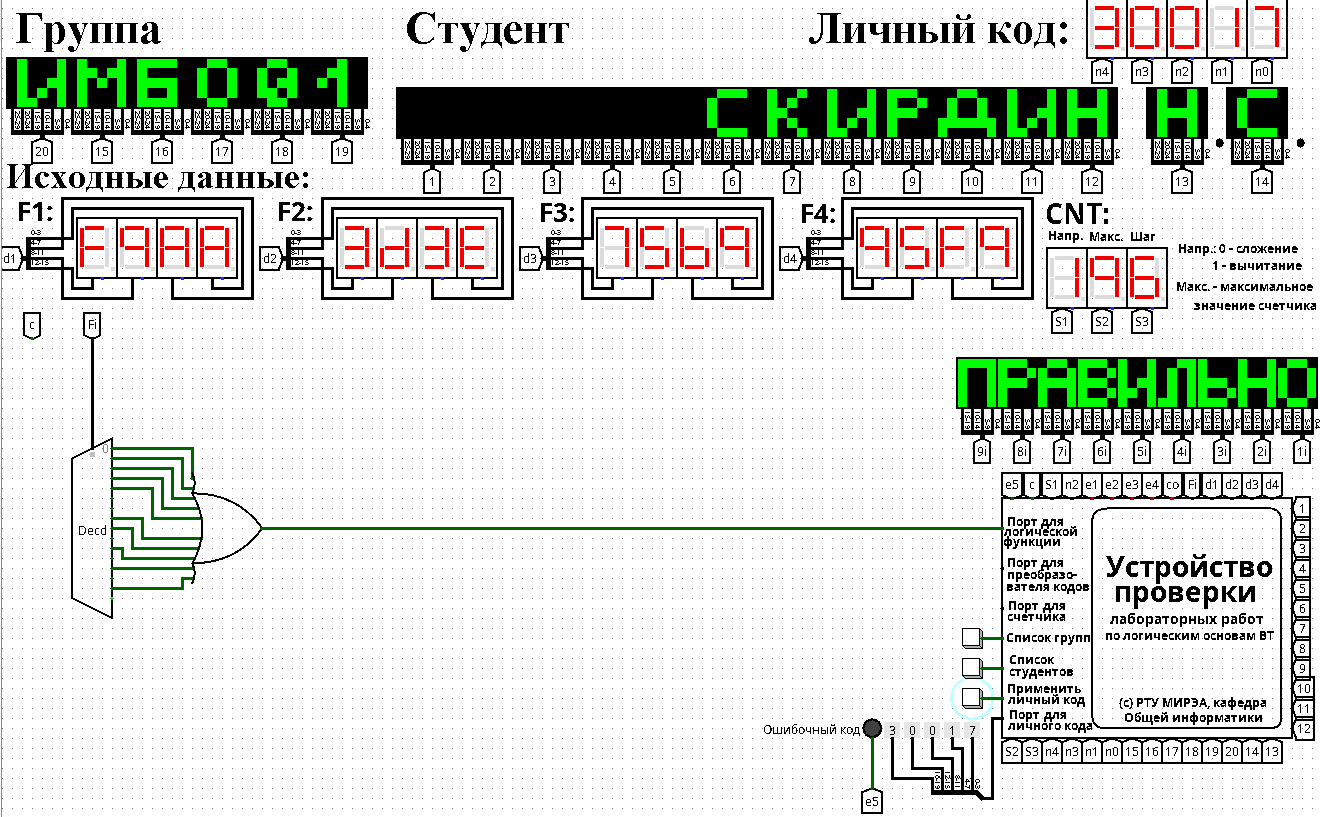
\includegraphics[width=\textwidth]{decoder-4-16}
\end{figure}

\section{Реализация функции с использованием двух дешифраторов 3-8 и необходимой дополнительной логикой}
Реализуем функцию, используя дешифраторы 3-8 и необходимую дополнительную логику. Количество выходов у дешифратора 3-8 в два раза меньше количества значений логической функции, поэтому нам потребуется разместить на рабочей области лабораторного комплекса два дешифратора 3-8. Также следует обратить внимание, что количество адресных входов дешифратора меньше, чем количество переменных функции, поэтому подадим значения трех младших переменных функции на адресные входы обоих дешифраторов: младшую переменную «d» — на младший адресный вход, старшую переменную «b» — на старший адресный вход, переменную «с» — аналогично (на схеме далее переменные подаются на адресные входы дешифраторов при помощи разветвителя и шины).

Переменная «а» используется для управления дешифраторами. Когда «а» равна нулю, то должен работать первый дешифратор - он отвечает за первую половину таблицы истинности. Когда «а» равна единице, то должен работать второй дешифратор — он отвечает за вторую половину таблицы истинности. Чтобы это реализовать, переменная «а» должна подаваться на разрешающий вход первого дешифратора через инверсию, а на вход второго — без инверсии.

В процессе работы на выходах всех дешифраторов будут последовательно возникать единичные значения в соответствии с поступающей на адресные входы комбинацией значений переменных. У первого дешифратора выберем лишь те выходы, чьи номера совпадают с номерами наборов значений переменных, на которых функция равна единице, из первой половины таблицы. У второго дешифратора выберем лишь те выходы, чьи номера совпадают с номерами наборов значений переменных за вычетом 8, на которых функция равна единице, из второй половины таблицы.

Объединим выбранные выходы обоих дешифраторов через «или» и получим требуемую реализацию (\cref{fig:decoder-3-8}).
\begin{figure}[H]
	\caption{Тестирование схемы, реализующей логическую функцию на дешифраторах 3-8 и дополнительной логике}
	\label{fig:decoder-3-8}
	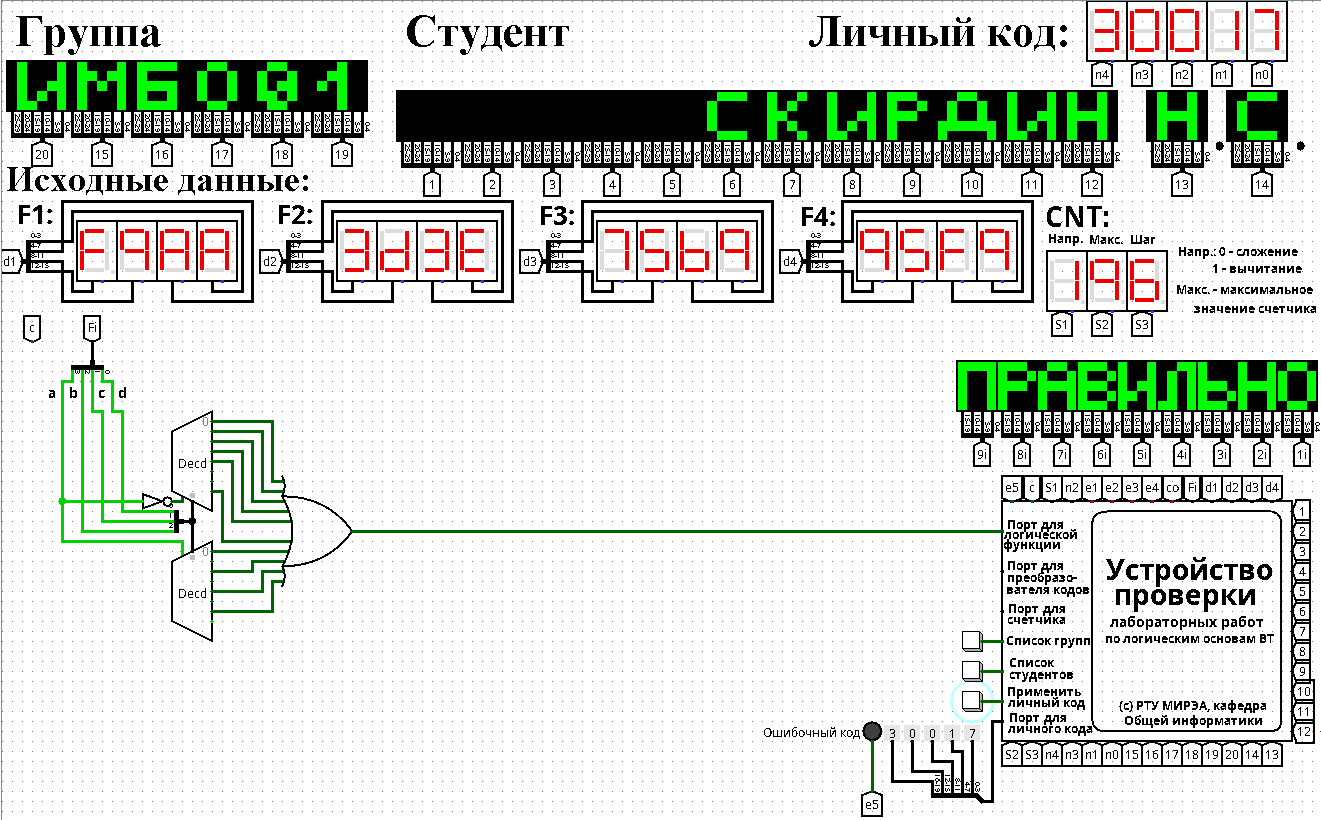
\includegraphics[width=\textwidth]{decoder-3-8}
\end{figure}

\section{Реализация функции с использованием пяти дешифраторов 2-4 и одной дополнительной схемой «или»}
Реализуем функцию, используя дешифраторы 2-4 и необходимую дополнительную логику. Количество выходов у дешифратора 2-4 в четыре раза меньше количества значений логической функции, поэтому нам потребуется разместить на рабочей области лабораторного комплекса четыре дешифратора 2-4, которые мы будем называть операционными, а также еще один дешифратор 2-4, который будет управлять первыми четырьмя – назовем его управляющим.

Итого всего потребуется пять дешифраторов 2-4 и дополнительная схема
«или».

Следует обратить внимание, что количество адресных входов у каждого дешифратора в два раза меньше, чем количество переменных функции, поэтому каждый операционный дешифратор будет отвечать лишь за одну четверть исходной таблицы истинности.

Значения двух младших переменных функции используются для адресации четырех операционных дешифраторов: младшая переменная «d» - подается на младший адресный вход, старшая переменная «с» - на старший адресный вход (на схеме далее переменные подаются на адресные входы дешифраторов при помощи разветвителя и шины).

Переменные «а» и «b» используются для управления операционными дешифраторами и аналогичным образом подаются на адресные входы управляющего дешифратора. Выходы управляющего дешифратора должны быть подключены к разрешающим входам операционных дешифраторов. Таким образом, когда «а» и «b» равны нулю, то на нулевом выходе управляющего дешифратора образуется единица, которая подается на разрешающий вход первого операционного дешифратора и так далее.

Теперь фактически каждый операционный дешифратор отвечает за свою двоичную тетраду в исходной векторной записи логической функции. Выберем у каждого операционного дешифратора лишь те выходы, где у двоичной тетрады стоят единицы. При этом необходимо считать, что нулевой выход соответствует старшему двоичному разряду тетрады.

Объединим выбранные выходы всех операционных дешифраторов через «или» и получим требуемую реализацию (\cref{fig:decoder-2-4}).

\begin{figure}[H]
	\caption{Тестирование схемы, реализующей логическую функцию на дешифраторах 2-4 и дополнительной логике}
	\label{fig:decoder-2-4}
	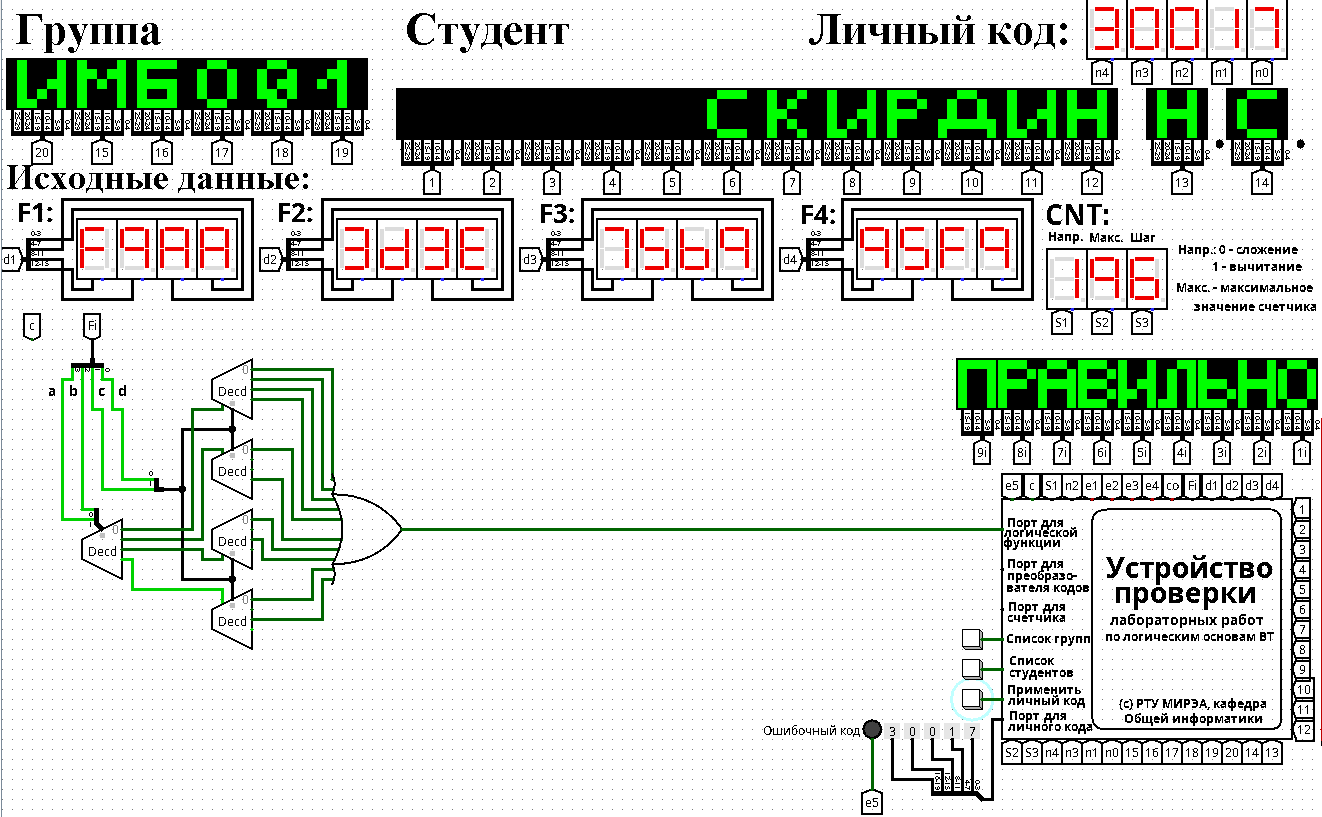
\includegraphics[width=\textwidth]{decoder-2-4}
\end{figure}

\chapter{Выводы}
В ходе работы была восстановлена таблица истинности логической функции от четырех переменных. По таблице истинности были реализованы в лабораторном комплексе логические функции на дешифраторах тремя способами:

– используя дешифратор 4-16 и одну дополнительную схему «или»;

– используя два дешифратора 3-8 и необходимую дополнительную логику;

– используя пять дешифраторов 2-4 и одну дополнительную схему «или».

Работа схем была протестирована, чтобы убедиться в правильности их работы.

\chapter{Информационный источник}
\textbf{Смирнов, С. С.} Информатика : Методические указания по выполнению практических работ / С. С. Смирнов, Д. А. Карпов. -- Москва : МИРЭА -- Российский технологический университет, 2020. -- 102 с.

\end{document}
